\part{Cours Magistral 5 -- Les intégrales}
Ce cours couvre le chapitre 16 du livre de référence.

\section{Analyse Vectorielle}


Nous allons travailler essentiellement en 2D et 3D. Certaines propriétés peuvent être étendues mais pas toutes. Dans ce cours $rot$, $grad$ et $div$ sont tous les trois des vecteurs.

\subsection{Gradient, divergence, rotationnel ; opérateurs différentiels}
\subsubsection{Gradient d'un scalaire f (x,y,z)}

$grad f = \nabla f$ = opérateur "del", "nabla", "gradient" appliqué à $f$.

$grad f = \nabla f =\frac{\partial f}{\partial x} i +\frac{\partial f}{\partial y} j +\frac{\partial f}{\partial z} k$

\[\nabla \star = \frac{\partial \star}{\partial x} i +\frac{\partial \star}{\partial y} j +\frac{\partial \star}{\partial z} k\]
\subsubsection{Divergence}
\begin{mydef}
La divergence d'un vecteur se définit par
\[div F = \vec \nabla \bullet \vec F\]
Le résultat de ce calcul est un scalaire
\[div F = \left( \frac{\partial \star}{\partial x} i +\frac{\partial \star}{\partial y} j +\frac{\partial \star}{\partial z} k \right) \bullet (F_1 i +F_2 j +F_3 k) \]

\[= i\bullet i \frac{\partial F_1}{\partial x}+j\bullet j \frac{\partial F_2}{\partial y}+k\bullet k \frac{\partial F_3}{\partial z}  \]

On trouve donc

\[div F = \frac{\partial F_1}{\partial x}+\frac{\partial F_2}{\partial y}+\frac{\partial F_3}{\partial z}\]
\end{mydef}

\subsubsection{Rotationnel}
\begin{mydef}
\[\textit{rot}F = \textit{ curl}F = \nabla \times F\]
C'est un produit vectoriel, le résultat est un vecteur.

\[=
\left|
\begin{array}{c c c}
i&j&k\\
\frac{\partial \star}{\partial x} & \frac{\partial \star}{\partial y} &\frac{\partial \star}{\partial z} \\
F_1& F_2&F_3
\end{array}
\right|
\]


\[\textit{F} = \left( \frac{\partial \star}{\partial x} i +\frac{\partial \star}{\partial y} j +\frac{\partial \star}{\partial z} k \right) \times  (F_1 i +F_2 j +F_3 k) \]

\[=\left( \frac{\partial F_3}{\partial y } -  \frac{\partial F_2}{\partial z }\right) i
+\left( \frac{\partial F_1}{\partial z } -  \frac{\partial F_3}{\partial x }\right) j
+\left( \frac{\partial F_2}{\partial x } -  \frac{\partial F_1}{\partial y }\right) i
\]

Pour un champ bidimensionnel on obtient toujours un vecteur perpendiculaire au plan xy.
\end{mydef}




\begin{myrem}

Attention, l'ordre des facteurs est important !
\[\nabla \bullet F = \frac{\partial F_1}{\partial x}+ \frac{\partial F_2 }{\partial y}+ \frac{\partial F_3 }{\partial z}\] C'est un scalaire

\[F\bullet \nabla = F_1  \frac{\partial \star }{\partial x}+F_2 \frac{\partial \star }{\partial y}+ F_3  \frac{\partial \star }{\partial z}\]

 \end{myrem}

\subsubsection{Exemple :}

\[F=(xy)i+(y^2-z^2)j+(yz)k\]

\[\nabla \bullet F = \textit{div } F = \frac{\partial }{\partial x} ( (xy)+\frac{\partial }{\partial y} (y^2-z^2)+\frac{\partial }{\partial z} (yz) = y+2y+y=4y\]

\[\textit{rot }F = \left( \frac{\partial }{\partial z} (xy) -\frac{\partial }{\partial x} (yz) \right) j
+\left( \frac{\partial }{\partial z} (yz) -\frac{\partial }{\partial z} (y^2-z^2) \right)
 \]



 \subsection{Identités reliant grad, div et rot}

 Cf. Adams p897 Section 16.2

 Exemple :

 \[\nabla \bullet ( F \times G) = ( \nabla \times F) \bullet G - F \bullet(\nabla \times G ) \]

 On peut vérifier qu'il s'agit bien de scalaires. Il y a une infinité de formules les reliant mais on doit en connaître uniquement deux.

 \begin{itemize}
 \item
 \[\textit{div}(\textit{rot } F ) = 0 = \nabla \bullet ( \nabla \times F ) \]
\textit{Démonstration :} \\

 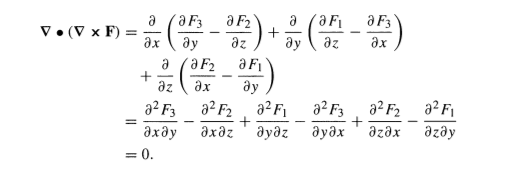
\includegraphics[scale=0.7]{image1.png}

 Tous les termes s'annulent deux à deux.
 \item
 \[\textit{rot} ( \textit{grad }\phi) =0 = \nabla \times ( \nabla \phi ) \]

 \end{itemize}
 \subsection{Terminologie}
\begin{itemize}


\item
 $div F = 0$ dans $D \Leftrightarrow F$ est un champ vectoriel " solénoïdal " ou encore " incompressible " dans D;

\item $rot F = 0$ dans $D \Leftrightarrow F$ est un champ vectoriel " irrotationnel " dans $D$.

\end{itemize}
\textit{ Exemples physiques :} \\

 $\vec F= \vec B$ (le champ magnétique). $div B = 0$

 $\vec F= \vec V$ (la vitesse du fluide). $div V = 0$

 Si le fluide est incompréssible $\Leftrightarrow$ Densité constante (m/vol).
 
 \textit{ Exemple} :

 \[F= grad \phi = \nabla \phi \textit{ (conservatif) }\]

 \[rot F = rot ( grad \phi ) =0\]

 \begin{mytheo}
 Un champ de vecteurs conservatif est irrotationnel.
 \end{mytheo}

 \[div ( rot G ) = 0\]

 Si on appelle $rot G = F$.

 \begin{mytheo}
 Le rotationnel d'un champ vectoriel est solénoïdal/incompressible.
 \end{mytheo}


 \begin{mytheo}
 C'est la réciproque du théorème 1.


 Un champ de vecteurs irrotationnel est conservatif.
 \end{mytheo}


 \begin{mytheo}
C'est la réciproque du théorème 2.

 Un champ vectoriel solénoïdal ou incompressible dérive d'un potentiel vecteur : $\exists G \textit{ tel que } \vec F = rot \vec G$.
 \end{mytheo}
 \begin{myrem}

Pour prouver qu'un champ vectoriel est un grand $\vec f $ tel que $\vec f = grad F$, il faut que le domaine soit simplement connexe et que $rot F=0$. Pour vérifier cela, il suffit d'utiliser la définition du $rot$.

 \end{myrem}
 Ces réciproques sont vraies si le domaine D de définition du champ $\vec F$ satisfait à certaines conditions. Les réciproques ne sont pas toujours vraies, quel que soit le domaine.

 Nous allons démontrer que les réciproques sont vraies pour D = ouvert, simplement connexe, \textbf{étoilé}


 \textit{Réciproque du Théorème 1} : Hypothèse : $rot \vec F =0$

 \[rot \vec F
=\left( \frac{\partial F_3}{\partial y } -  \frac{\partial F_2}{\partial z }\right) i
+\left( \frac{\partial F_1}{\partial z } -  \frac{\partial F_3}{\partial x }\right) j
+\left( \frac{\partial F_2}{\partial x } -  \frac{\partial F_1}{\partial y }\right) i
\]

 On suppose que chaque composante est nulle.

 Donc,
 \[\frac{\partial F_i}{\partial x_i}=\frac{\partial F_j}{\partial x_j}\]


Cf. les conditions évoquées dans le théorème de Poincaré. Donc, si on parvient à démontrer la réciproque du théorème 1, on aura démontré le théorème de Poincaré.

D doit être ouvert simplement connexe pour que Poincaré soit vrai.\\




\textit{
Démonstration constructive :}
\textit{
Hypothèse :}

\begin{itemize}
\item F  irrotationnel $\Leftrightarrow rot F =0$;
\item D ouvert, simplement connexe, étoilé.
\end{itemize}

\begin{mydef}[Un domaine étoilé]

$\exists P_0 \in D : \forall P \in D $ le segment de droite $(P_0+t( P-P_0))$, avec $t\in [0,1]$ est entièrement contenu dans D. Voir image.\\

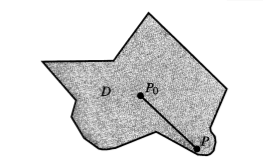
\includegraphics[scale=1]{image2.png}\\
\end{mydef}

$P_0 = (0,0,0)$ ; $\vec r(t) = (tx)i + (ty) j +(tz) k$

$P=(x,y,z)$

On doit montrer que F est conservatif. $\exists \phi : \vec F = \nabla \phi $

\[\Leftrightarrow F_1=\frac{\partial \phi}{\partial x}; F_2=\frac{\partial \phi}{\partial y};F_3=\frac{\partial \phi}{\partial z}\]

$\forall(x,y,z)\in D$

\[\phi(x,y,z) = \int_{P_0-P} \vec F \bullet \vec dr \] On a supposé que le domaine était étoilé.

\[\phi(x,y,z) = \int _{t=0} \left( F\bullet \frac{dr}{dt} dt \right) \]

\[\frac{dr}{dt} = (x) i +(y)j +(z) k\]

On pose $\alpha = tx$; $\beta = ty $ ; $\gamma = tz$

Dans le livre, il y a d'autres notations.

Notons que $\frac{\partial \alpha}{\partial t} = x$

On a donc

\[\phi (x,y,z) = \int_0^1 \left( x F_1 (\alpha, \beta, \gamma ) + y F_2 + z F_3 \right) dt \]

On va calculer

\[\frac{\partial \phi}{\partial x} = \int_0^1 \frac{\partial}{\partial x} \left( x F_1 (\alpha, \beta, \gamma ) + y F_2 + z F_3 \right) dt\]

\[= \int_0^1 \left( 1F_X +X \frac{\partial F_1}{\partial x} + y \frac{\partial F_2}{\partial x} + z \frac{\partial F_3}{\partial x} \right) dt\]


\[
\frac{\partial F_1}{\partial x} = \frac{\partial F_1}{\partial \alpha} \frac{\partial \alpha}{\partial x}
=\frac{\partial F_1}{\partial \beta} \frac{\partial \beta}{\partial x}
=\frac{\partial F_1}{\partial \gamma} \frac{\partial \gamma}{\partial x}
\]

Or on a,

\[\frac{\partial F_1}{\partial x} = t \frac{\partial F_1}{\partial \alpha}\]

\[\frac{\partial F_2}{\partial x} = t \frac{\partial F_2}{\partial \alpha}\]

\[\frac{\partial F_3}{\partial x} = t \frac{\partial F_3}{\partial \alpha}\]

On trouve donc

\[\frac{\partial \phi}{\partial x}=\int_0^1 \left( F_1+t \frac{\partial F_1}{\partial \alpha} \frac{\partial \alpha}{\partial t}
+t \frac{\partial F_2}{\partial \alpha} \frac{\partial \\beta}{\partial t}
+t \frac{\partial F_3}{\partial \alpha} \frac{\partial \gamma}{\partial t}
\right) dt
\]

Cependant, par hypothèse, $rot \vec F = 0$

\[\Leftrightarrow  \frac{\partial F_2}{\partial \alpha} = \frac{\partial F_1}{\partial \beta} \text{ et }  \frac{\partial F_3}{\partial \alpha} = \frac{\partial F_1}{\partial \gamma} \]

On trouve alors

\[
\frac{\partial \phi}{\partial x}=\int_0^1 \left( F_1 +t \frac{\partial F_1}{\partial \alpha} \frac{\partial \alpha}{\partial t}
+t \frac{\partial F_1}{\partial \beta} \frac{\partial \\beta}{\partial t}
+t \frac{\partial F_1}{\partial \gamma} \frac{\partial \gamma}{\partial t}
\right) dt
\]

\[=\int_0^1 \frac{d}{dt}[t F_1 ( \alpha, \beta, \gamma ) ] dt \]

On peut démontrer aussi pour $F_2 $ et $F_3$

\[ = tF_1 ( tx,ty,tz) \textit{entre 0 et 1} = F_1 (x,y,z) - 0\]

\begin{myrem}

Théorème 2 : Si G est un potentiel vecteur de $\vec F$, alors $(G+\nabla \phi )$ l'est aussi. $\nabla \phi$ est un champ de vecteurs conservatif.
$rot ( G+\nabla \phi )  = rot G + rot ( \nabla  \phi )$ avec $rot ( \nabla  \phi )=0$
\end{myrem}


Le potentiel vecteur est défini à un vecteur conservatif près.

\section{Les Théorèmes Intégraux}


Voici les trois raisons pour lesquelles on voit ces théorèmes :
\begin{itemize}
\item Utiles et fondamentaux pour la suite (``physique des milieux continus'');
\item Permettent de donner une interprétation intuitive à $div$ et $rot$;
\item Permettent de passer d'un type d'intégrale à un autre. Par exemple, d'une intégrale de surface à une intégrale de contour.
\end{itemize}

Ce sont des cas particuliers d'un théorème unique dans le cadre de la théorie des formes différentielles extérieures.

\subsection{Théorème de Green dans le plan xy}

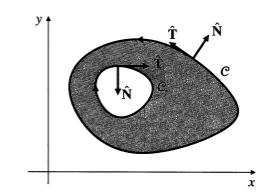
\includegraphics[scale=1]{image3.png}
\\
R est une surface orientée $ \hat N = \vec k$ et C = bord orienté.

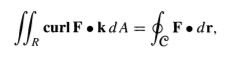
\includegraphics[scale=0.7]{image4.png}\\

\[F=F_1(x,y)i+F_2(x,y)j\]

On peut réécrire le Théorème de Green comme ceci\\
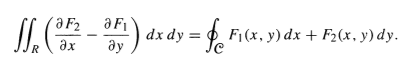
\includegraphics[scale=0.7]{image5.png}\\
\textit{
Exemple 1 : }

$\vec F=xj$ (1), $\vec F = -y i$(2) et $\vec F = 0.5 ( -y i +x j )$ (3)

Pour les trois exemples, on obtient \[\frac{\partial F_2}{\partial x}- \frac{\partial F_1}{\partial y} = 1\]

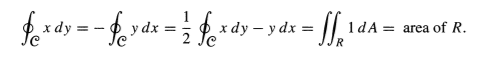
\includegraphics[scale=0.7]{image6.png}\\

Merci Green !

Appliqué à un disque elliptique :

\textit{
Exemple 2 : }\\
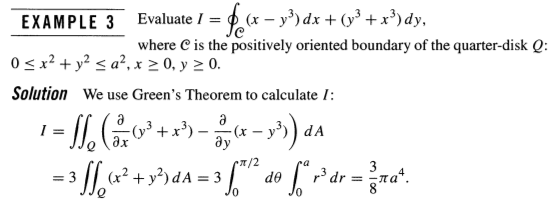
\includegraphics[scale=0.7]{image7.png}\\

\begin{myrem}

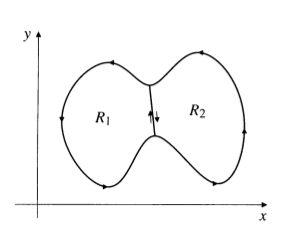
\includegraphics[scale=0.8]{image8.png}

\[\int_+ F\bullet dr = - \int_- F\bullet dr\]

Si on considère l'union des deux domaines, le Théorème de Green est valable sur l'union des deux domaines. En fait, on a fait une \textbf{coupure fictive de $R$}.
\end{myrem}
